

\documentclass[10pt,journal,letterpaper,compsoc]{IEEEtran}
\usepackage{cite}
\usepackage{url}
\usepackage{times}
\usepackage{graphicx}
\usepackage{url}
\usepackage{clrscode}
\usepackage{tabularx}
\usepackage{amsmath}
\usepackage{array}
\usepackage{color}
\usepackage{balance}

\begin{document}

\title{An Implementation of the Active Contours without Edged model and the Logic Framework for Active contours on multi-channel images}

\author{Karim Ali and Sarah Nadi\\
\{karim, snadi\}@cs.uwaterloo.ca \\
David R. Cheriton School of Computer Science\\
University of Waterloo\\
}



% The paper headers
\markboth{CS870 Project Report - Active Contour without Edges}%
{Shell \MakeLowercase{\textit{et al.}}: Bare Demo of IEEEtran.cls for Computer Society Journals}


\IEEEcompsoctitleabstractindextext{%
\begin{abstract}
%\boldmath
The abstract goes here.
\end{abstract}
}

\maketitle



\section{Introduction}
Image segmentation or boundary detection is a very important problem in the area of Image Processing, and has received a lot of attention in the past. The
classical Active Contour model (or Snakes) proposed by Kass et al.~\cite{kass1988snakes} was the first model to use the idea of energy minimization to attract
a contour to the edges of the objects in an image. The Snakes model was very successful and variations of it very highly adopted later on
(E.g.~\cite{caselles1997geodesic}. Most of these models used the level set formulation for propagating fronts to evolve the curve. However, these models highly
depended on curvature motion (motion defined by the gradient of the curve) which led to poor performance in smoothed edges. To overcome these limitations, Chan
and Vese~\cite{chan2001active} propose an active contour model that does not depend on the edges (i.e the gradient) for propagating the curve to detect the
boundary of the object. Instead, they use a region-based approach based on the Mumford-Shah model~\cite{mumford1989optimal} to divide the image
into two regions: one inside the propagating curve, and one outside. The curve is at the boundary of the object if there is no difference in intensities inside
the curve as well as outside the curve.

The Active Contours without Edges model proposed by Chan and Vese (referred to as Chan-Vese model throughout the rest of this paper) was very successful in
detecting objects even in noisy or blurry images. It could also detect holes in objects which was usually a limitation in previous models. As an extension to
this work, Sandberg and Chan~\cite{sandberg2005logic} propose a logic framework (referred to as the Sandberg-Chan model throughout the rest of this
paper) that  performs logical operations on multiple images according to the curve propagation proposed in the Chan-Vese model. To achieve that, previous models
usually had two steps. They would either first segment the object in each channel separately then combine the segmented objects according to the logic operation
through bitwise operations (CITE) or they would apply logic operations to the different images then segment the resulting image (CITE). The first approach is
very costly, and the second approach requires a lot of prior knowledge about the intensities of each image. To overcome these drawbacks, the Sandberg-Chan
model is based on the idea of fitting a single contour to the object on all channels according to the logic operator, and based on regions.

In this paper, we report on our findings after implementing each of these models. We implemented both models in Matlab, and experimented with several images.
In this paper, we explain the details of our implementation as well as our results. The rest of this paper is organized as follows: Section~\ref{sec:bg} first
provides brief background about each of the two models implemented in this paper. Section~\ref{sec:implementation} then explains our implementation. In this
section, we explain how we implemented the models and any variations from the original papers. Section~\ref{sec:results} explains our evaluation criteria, and
presents the results we obtained. Section~\ref{sec:difficulties} discusses some of the difficulties we faced, and points out some BLA. Section~\ref{sec:concl}
concludes this paper by summarizing our findings.


\section{Background}
\label{sec:bg}

\subsection{Chan-Vese Model}
\label{sec:chan-vese}

The Chan-Vese model is a region based model for detecting objects in an image. It is based on a restriction Mumford-Shah model which divides an image into
regions and represents each region by a piecewise constant (the minimal partition problem). Figure~\ref{fig:region} shows what is meant by a region based
model. The figure shows an image $u_{0}$ which has a gray triangular object in it. The red curve, C, is the initial contour used to detect this object. The
main idea behind the model is that the curve divides the image into two regions: that inside the curve and that outside. Each region is represented by a
constant, c, which is the average intensity of the image values in each region. In order for the curve to fit the object, there must be no variation of the
intensities inside the curve as well as outside. In other words, this turns into a minimization problem of the difference of intensities inside (fitting term
one, $F_{1}$) plus those
outside (fitting term two, $F_{2}$). For example, in the figure, the point $(x_{1},y_{1})$ will have to be outside the curve in order to minimize the difference
between the points inside
the curve. Similarly, the point $(x_{4}, y_{4})$ will have to be inside the curve. Figure~\ref{fig:fitting} shows all the possibilities of the curve's fitting
according to its position with respect to the object.

More formally, the Euler-Lagrange equation (as derived in the original paper) representing the time motion of the curve C is shown in Equation~\ref{eqn:cvpde}.

\begin{equation}
\label{eqn:cvpde}
\frac{\partial{\phi}}{\partial{t}} = \delta_{\varepsilon}(\phi)[\mu\; \mathrm{div}(\frac{\bigtriangledown \phi}{|\bigtriangledown \phi|}) - \nu -
\lambda_{1}(u_{0} - c_{1})^2 +\lambda_{2}(u_{0} - c_{2})^2] 
\end{equation}

\begin{figure}[t]
\centering
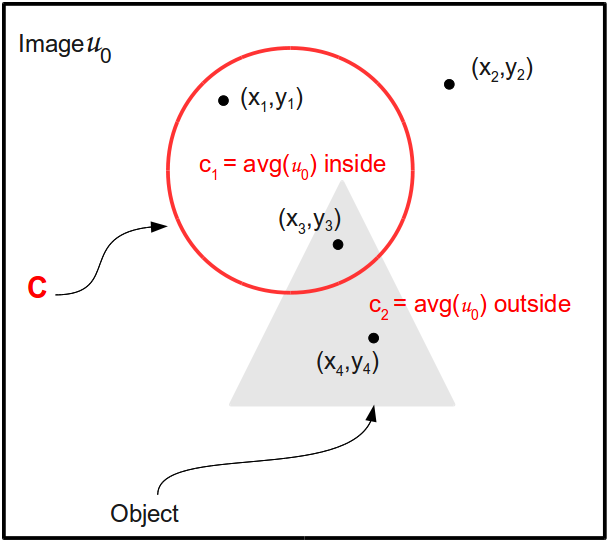
\includegraphics[width=6cm]{explaining.png}
\caption{Region Based Model}
\label{fig:region}
\end{figure}

(REST OF EQUATION HERE)

The parameter $\mu$ is a scaling parameter for the length of the curve represented in terms of curvature. The smalled $\mu$ is, the more the length of the curve
can increase without penalizing the minimization. This allows the model to detect smalled objects and holes. The larger $\mu$ is, the less freedom there is for
the curve to increase in length, and thus, it will only be able to detect larger objects. The parameter $\nu$ is also a scaling term for the area of the curve.
However, the authors do not use the area term in the Euler-Lagrange derivation, and always set $\nu$ to 0. It seems that $\mu$ is sufficient to scale the curve
according to the objects that need to be detected. Finally, $\lambda_{1}$ and $\lambda_{2}$ are weighting parameters for the forces inside the curve and
outside the curve respectively. Since we want to give both forces equal weight, the authors set $\lambda_{1} = \lambda_{2} = 1$ in all their experiments.



\subsection{Sandberg-Chan Model}
\label{sec:sandberg-chan}

The main goal of the Sandberg-Chan model~\cite{sandberg2005logic} is to perform logic operations on a combination of different images accurately and
efficiently. For example, finding the union of two images where different parts of the object are occluded in each image so that a complete object can be
obtained. In order to do that, they use the Chan-Vese model to detect objects, and simultaneously include the logic operations in the minimization problem.
Since they are using the Chan-Vese model, the problem must be viewed in terms of regions as well. Accordingly, they define the two main logic operations
(union and intersection) in terms of regions where the union of two images is the union of the insides of the curve with respect to the images plus the
intersection of the outsides of the curve with respect to the images. For example, Figure~\ref{fig:logic-op} (taken from the original paper) shows that the
union of $A_{1}$ and $A_{2}$ (in terms of its shape) can be obtained by taking the union of the insides of the object or the intersection of the outsides.
Similarly, the intersection of two images would be the intersection of the insides plus the union of the outsides. Thus, in order to obtain accurate results
irrespective of the object's intensity outside versus inside, we should consider \textit{both} the logical operation required for the region inside the object
as well as that outside.

\begin{figure}[t!]
\centering
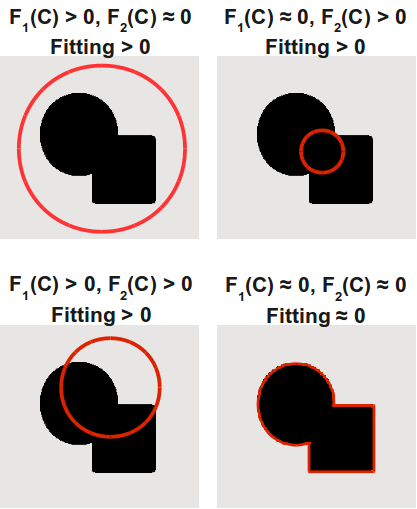
\includegraphics[width=6cm]{fitting.png}
\caption{Chan-Vese Curve Fitting}
\label{fig:fitting}
\end{figure}

More formally, the authors define two logic variables $z_{i}^{in}$ and $z_{i}^{out}$ to denote whether a point $(x,y)$ should be in the moving curve C or not
with respect to image i. Since we are trying to minimize the fitting of the curve, they use 0 to denote true and 1 to denote false (the reverse of the usual
convention. Following the Chan-Vese model, they represent each of the regions inside and outside the curve by a constant c. In this paper, they represent
$c_{in}$ as $c_{+}$ and $c_{out}$ as $c_{-}$. Equations~\ref{eqn:zin} and~\ref{eqn:zout} show how to calculate $z_{in}$ and $z_{out}$ respectively in terms of
the Chan-Vese model. We note here that in the original paper there was a typo in these equations where they divide by the maximum intensity of each image
instead of the maximum intensity squared. However, in order to have $z_{in}$ and $z_{out}$ have values from 0 to 1 that represent logic values, we need to
divide by the maximum intensity squared. The equations shown below have been corrected for that.

\begin{figure*}[t]
\centering
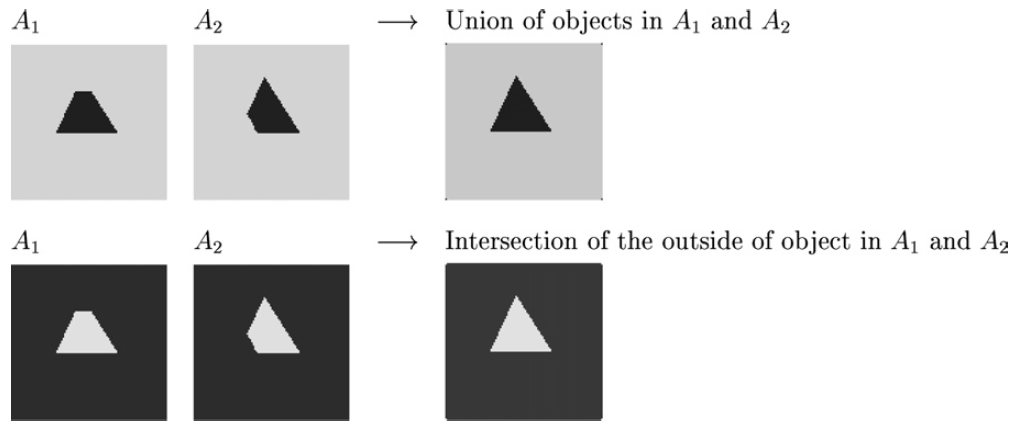
\includegraphics[width=12cm]{logicop.png}
\caption{Region Based View Union}
\label{fig:logic-op}
\end{figure*}

\begin{equation}
\label{eqn:zin}
z_{i}^{in}(u_{0}^{i},x,y,C) = \frac{|u_{0}^{i} - c_{+}^i|^2}{(max^{2}_{(x,y) \in u_{0}^{i}} u_{0}^i)^2}
\end{equation}

\begin{equation}
\label{eqn:zout}
z_{i}^{out}(u_{0}^{i},x,y,C) = \frac{|u_{0}^{i} - c_{-}^i|^2}{(max_{(x,y) \in u_{0}^{i}} u_{0}^i)^2}
\end{equation}

In order to perform logic operations on $z_{in}$ and $z_{out}$, the authors introduce interpolation functions that mimic the behavior of the regular truth
table, but for continuous values between 0 and 1. The union and intersection functions for two variables are shown in Equations~\ref{eqn:funion}
and~\ref{eqn:finters} respectively. These equations can be simply extended to any number of variables.

\begin{equation}
\label{eqn:funion}
f_{\cup} = (z_{1} . z_{2})^{1/2}
\end{equation}

\begin{equation}
\label{eqn:finters}
f_{\cup} = 1 = ((1 - z_{1}) .(1-  z_{2}))^{1/2}
\end{equation}

Based on these functions, the Euler-Lagrange equation for any logic operation is shown in Equation~\ref{eqn:svpde}. According to the desired logic operation,
$f_{in}$ and $f_{out}$ will be specified accordingly. For example, if we are doing the union of the images, then we will need to perform a union operation on
the insides. Thus, $f_{in}$ will be replaced by Equation~\ref{eqn:funion}. Similarly, we will need to do the intersection of the outsides so $f_{out}$ will be
replaced by Equation~\ref{eqn:finters}.

\begin{equation}
\label{eqn:svpde}
\frac{\partial{\phi}}{\partial{t}} = \delta(\phi)[\mu\bigtriangledown(\frac{\bigtriangledown \phi}{|\bigtriangledown \phi|})  - \lambda(f_{in}(z_{1}^{in}, ...,
z_{n}^{in}) - f_{out}(z_{1}^{out}, ..., z_{n}^{out})
\end{equation}

with the boundary condition

$\frac{\delta(\phi)}{|\bigtriangledown\phi|}\frac{\partial\phi}{\partial n^{\rightarrow}} = 0$

\section{Implementation}
\label{sec:implementation}


\section{Experimental Results}
\label{sec:results}

In order to make sure we correctly implemented the models, we had several evaluation criteria. Table~\ref{tab:criteria} summarizes these criteria, and explains
the goals of each. Some of these criteria apply for both models, while other apply to one or the other. For the rest of this section, we proceed by presenting
our experimental results for both models. For each model, we proceed in the order of these criteria starting with the simplest
cases, and incrementally challenging the model.

\begin{table*}[h!t!]
\centering
\begin{tabular}{ c | c |c}
\textbf{Criteria} & \textbf{Goal} & \textbf{Applies to Model}\\
\hline\hline
Detecting Boundaries & Ability to correctly detect object boundaries of simple objects& Both Models\\
\hline
Curve Position & Ability to correctly detect object boundaries irrespective of the initial curve position & Both Models\\
\hline
Detecting Holes & Ability to detect holes in objects, and not simply stop on outside boundary & Both Models\\
\hline
Blurred Images & Ability to correctly (as much as possible) detect object boundaries in blurred images & Both Models\\
\hline
Noisy Images & Ability to correctly (as much as possible) detect object boundaries in noisy images & Both Models\\
\hline
Union Operator & Ability to correctly obtain the union of two or more images & Sandberg-Chan\\
\hline
Intersection Operator & Ability to correctly obtain the intersection of two or more images & Sandberg-Chan\\
\hline
Complement & Ability to correctly obtain the union or intersection of two or more images containing complements & Sandberg-Chan\\
\hline
Parameter Settings & Ability to respond correctly to the different parameter settings & Both Models\\
\end{tabular}
\centering
\caption{Evaluation Criteria}
\label{tab:criteria}
\end{table*}

\subsection{Chan-Vese Model Results}

\subsubsection*{Successful Detection of Boundaries}

\subsubsection*{Independence of Initial Curve Position}

\subsubsection*{Successful Detection of Holes}

\subsubsection*{Reasonable Performance with Blurred Images}

\subsubsection*{Reasonable Performance with Noisy Images}

\subsubsection*{Successful Response to Parameter Settings}

\subsubsection*{Other Tests}

\subsection{Sandberg-Chan Model Results}

\subsubsection*{Successful Detection of Boundaries}

\subsubsection*{Independence of Initial Curve Position}

\subsubsection*{Successful Detection of Holes}

\subsubsection*{Reasonable Performance with Blurred Images}

\subsubsection*{Reasonable Performance with Noisy Images}

\subsubsection*{Union}

\subsubsection*{Intersection}

\subsubsection*{Complement}

\subsubsection*{Successful Response to Parameter Settings}

\subsubsection*{Other Tests}

\section{Difficulties and Discussion}
\label{sec:difficulties}

\section{Conclusion}
\label{sec:concl}
The conclusion goes here.




\bibliographystyle{IEEEtran}

\bibliography{references}



% insert where needed to balance the two columns on the last page with
% biographies
%\newpage

\end{document}



